\documentclass[11pt,a4paper]{article}

\usepackage[utf8]{inputenc}
\usepackage{url}
\usepackage[margin=1in]{geometry}
\usepackage{graphicx}

\title{GitHub Cheat Sheet}
\date{}
\author{Econ 213R - Applied Machine Learning}

\begin{document}
\vspace*{-75pt}
    {\let\newpage\relax\maketitle}
    
\tableofcontents
    
\section{What is GitHub?}
GitHub is a place where developers can store projects and collaborate with other developers to create and update code.
Below is a list of terms you should know before you get started with GitHub.

\begin{itemize}
\item \textbf{repository}: place where all folders and files for a project are stored
\item \textbf{push}: update changes to a repository
\item \textbf{pull}: retrieve and merge changes to a repository
\item \textbf{commit}: an individual revision to a file or a set of files
\item \textbf{branch}: a parallel version of the repository contained within the repository but not affecting the primary branch (which is most often the master branch)
\item \textbf{clone}: a copy of a repository on your local machine
\item \textbf{fork}: a personal copy of another user's repository
\end{itemize}

Some of these definitions came from \url{https://help.github.com/articles/github-glossary/}, a useful guide for many GitHub terms.
    
\section{GitHub Registration}
You need an account with GitHub.
Go to \url{www.github.com}. 
Sign up from the home page and follow the instructions.
Note that private repositories require monthly payments; however, you can have an unlimited number of public repositories for free.
Once you sign up, you are ready to create and fork repositories.

\section{Creating Repositories}
Navigate to your GitHub profile.
It should look something like Figure \ref{fig:init-prof}.

\begin{figure}[h]
\centering
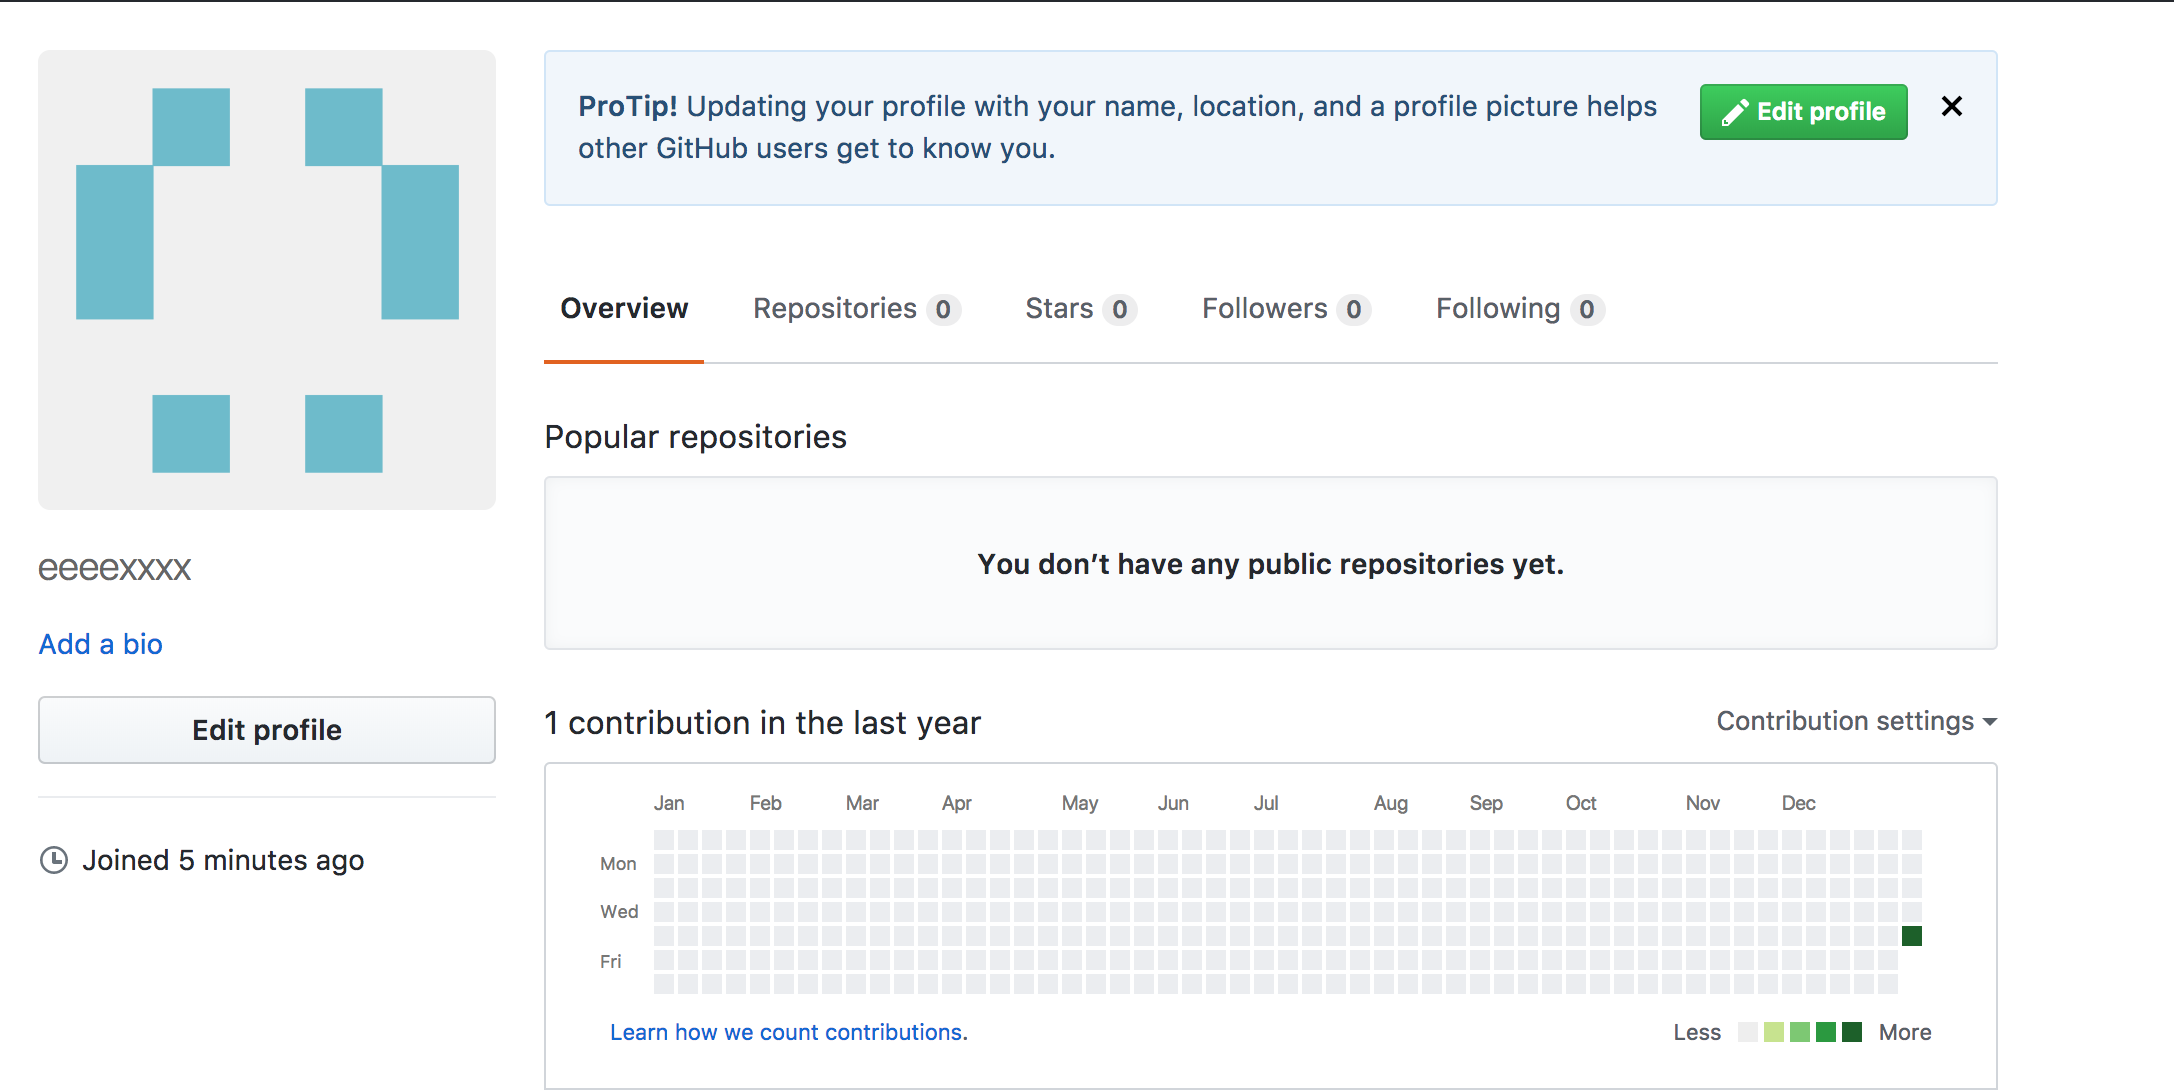
\includegraphics[width=.7\textwidth]{figures/init_profile.png}
\caption{Profile Screen}
\label{fig:init-prof}
\end{figure}

Click the ``Repositories" tab.
Click the button that says ``New" (see Figure \ref{fig:new-repo}).

\begin{figure}[h]
\centering
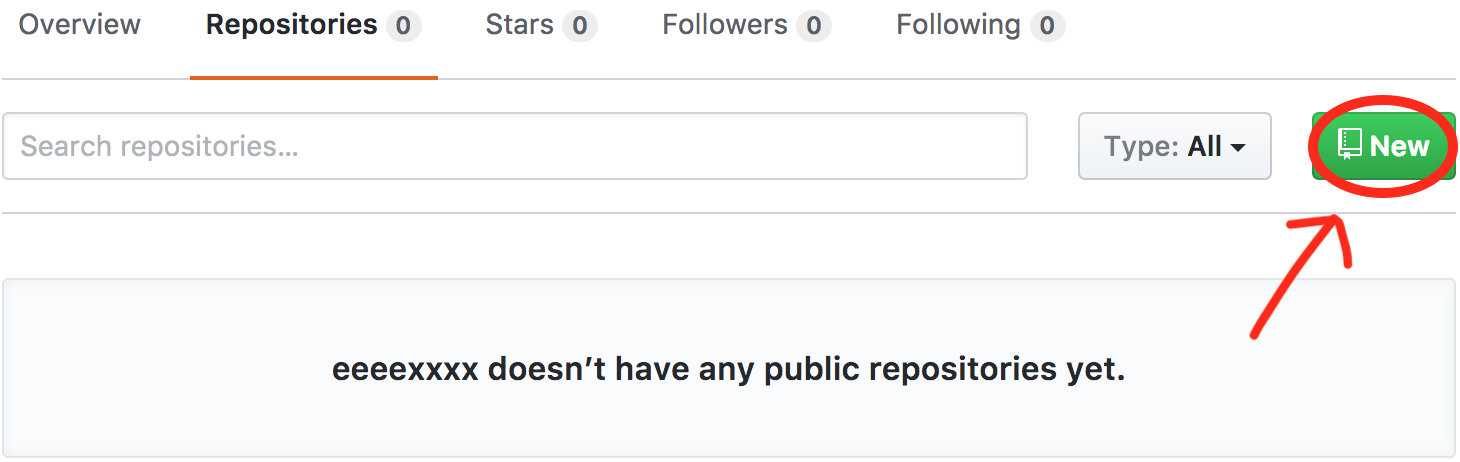
\includegraphics[width=.7\textwidth]{figures/new_repo.png}
\caption{New Repository}
\label{fig:new-repo}
\end{figure}

Name your repository.
It is customary to use dashes instead of underscores in repository names.
Make sure to initialize the repository with a README.md (see Figure \ref{fig:init-repo}).
If you accidentally forget to do this, that's okay; you can always add a README later.
A README is a short description of the repository.

\begin{figure}[h]
\centering
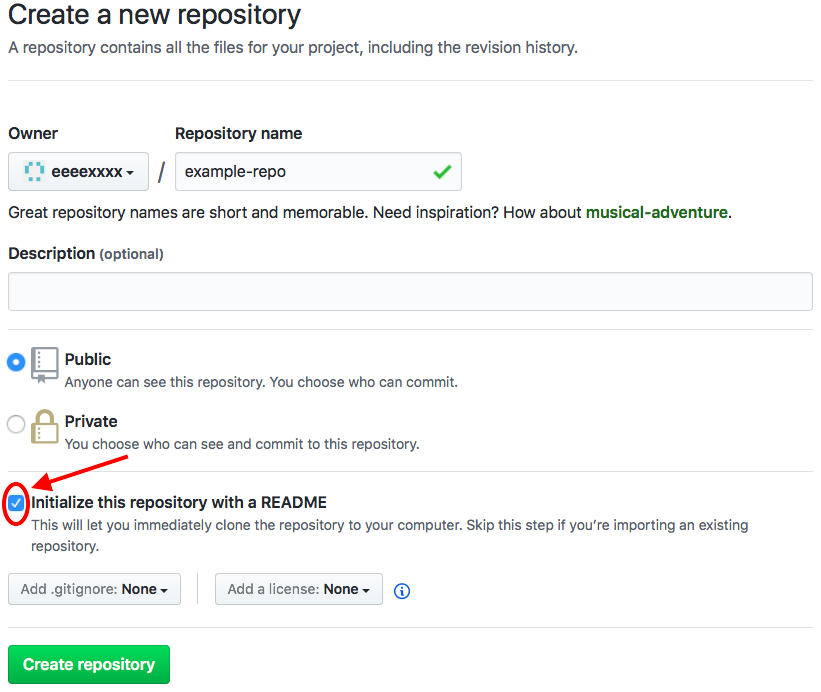
\includegraphics[width=.7\textwidth]{figures/init_repo.png}
\caption{Initialize the repository.}
\label{fig:init-repo}
\end{figure}

Click ``Create Repository" at the bottom of the page.
You should see a page that looks like Figure \ref{fig:repo-screen}.

\begin{figure}[h]
\centering
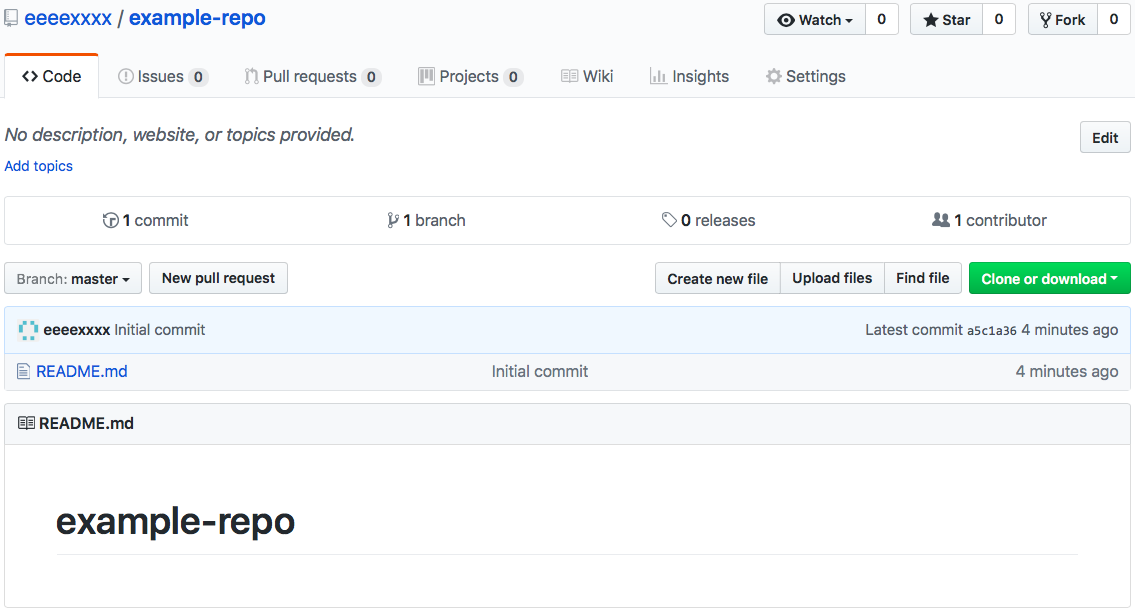
\includegraphics[width=.7\textwidth]{figures/repo_screen.png}
\caption{Repository screen.}
\label{fig:repo-screen}
\end{figure}

Congratulations!
You have just created your first GitHub repository.

\section{Making Changes to Repositories}
There are a few ways to upload and change files in a GitHub repository.
The most common way to modify repositories is via the command line; see Section \ref{command-line} for command line instructions.
It is highly, \textit{highly} recommended that you learn the command line to modify repositories.
The command line allows you to more freedom to modify your repositories and branches, and can streamline your workflow.
However, you can use the GitHub website to upload and download files to and from repositories.
You can also modify files using the website.
Note that you can't run Jupyter notebooks on the GitHub website, and when you try to edit Jupyter notebooks on the website, you have to comb through lots of nasty JSON lingo.
If you choose to use the website to make changes to the GitHub repository, you will have to download the Jupyter notebook, modify it on a local machine, and upload it back to the repository.
Instructions for using the website are in Section \ref{website}.

If you do not have Git installed on your local machine, use the links below to download Git.
\begin{itemize}
\item[] Macs: \url{https://sourceforge.net/projects/git-osx-installer/files/}
\item[] Windows: \url{http://gitforwindows.org/}
\item[] Linux: In the Terminal, first type \texttt{sudo apt-get update} and hit Enter. Then type \texttt{sudo apt-get install git} and hit Enter.
\end{itemize} 

\subsection{Using Command Line} \label{command-line}
Let's walk through an example together.
In this example, we will configure Git on a local machine, clone the repository to a local machine, create a Jupyter notebook, add it to the repository, and push the changes.

First, set your username and email in Git.
Use the commands below to do this.

\begin{itemize}
\item[] \texttt{git config --global user.name "Your Name Here"}
\item[] \texttt{git config --global user.email "your\_email@website.com"}
\end{itemize}

Now Git is configured on your machine, and you are ready to clone the repository you made.
First, go to the repository screen on the GitHub website (Figure \ref{fig:repo-screen}).
Click the button that says ``Clone or download".
A drop-down window should appear that contains a link to your repository (see Figure \ref{fig:clone-screen}).
Copy the link in the drop-down window.

\begin{figure}[h]
\centering
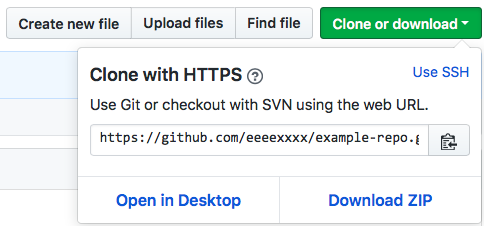
\includegraphics[width=.7\textwidth]{figures/clone_screen.png}
\caption{Jupyter notebook screen.}
\label{fig:clone-screen}
\end{figure}

Now open your command line.
Navigate to the location where you want your repository to be (for example, I store all of my files on my desktop, so I would navigate to my desktop from my command line).
Once you have navigated to the location, type the following command: \texttt{git clone link\_to\_your\_repo}, where \texttt{link\_to\_your\_repo} is the link you copied above..
When your computer is done downloading the repository, you should see a folder with the repository name in the location where you wanted it.
Now you are ready to make some changes and push them to your master branch.

\subsubsection{Making Changes}
For this example, we will make a Jupyter notebook and push it to the master branch.
In the command line, navigate to your repository if you're not there already.
Type \texttt{jupyter notebook} and hit enter.
A web browser should open up with a page that looks like Figure \ref{fig:jupyter-dir}.
If a web browser did not automatically open, the command line should have provided a URL that you can copy and past directly into a browser to access the Jupyter notebook.

\begin{figure}[h]
\centering
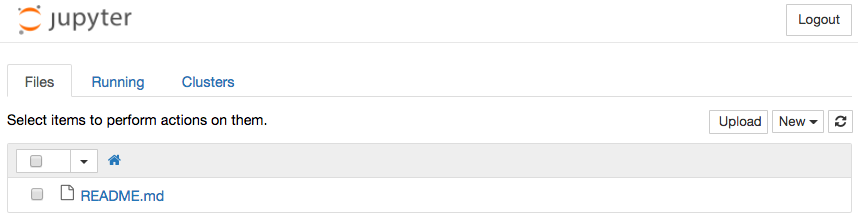
\includegraphics[width=.7\textwidth]{figures/jupyter_dir.png}
\caption{Jupyter notebook main screen.}
\label{fig:jupyter-dir}
\end{figure}

In the upper right-hand corner, click ``New".
A dropdown menu will appear.
Under the ``Notebooks" heading, click on Python 3 (see Figure \ref{fig:jupyter-dropdown}).
When you click ``Python 3", a new window will open in your browser with a screen that looks like Figure \ref{fig:jupyter}.

\begin{figure}[h]
\centering
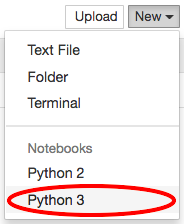
\includegraphics[width=.3\textwidth]{figures/jupyter_dropdown.png}
\caption{Create a Python 3 Jupyter notebook.}
\label{fig:jupyter-dropdown}
\end{figure}

\begin{figure}[h]
\centering
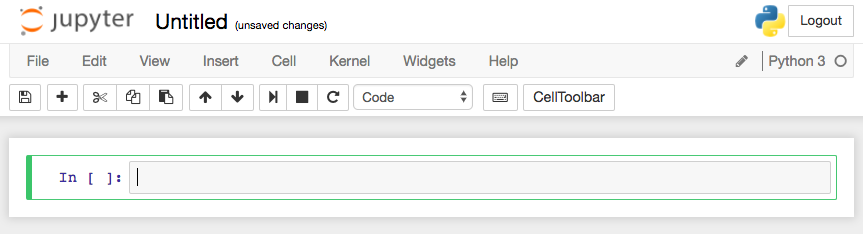
\includegraphics[width=.7\textwidth]{figures/jupyter.png}
\caption{A Jupyter notebook.}
\label{fig:jupyter}
\end{figure}

Change the name of the notebook from``Untitled" to ``example".
To do this, click the ``Untitled" text at the top of the notebook.
A window will appear; replace the ``Untitled" text with ``example".
See Figure \ref{fig:rename-notebook}.

\begin{figure}[h]
\centering
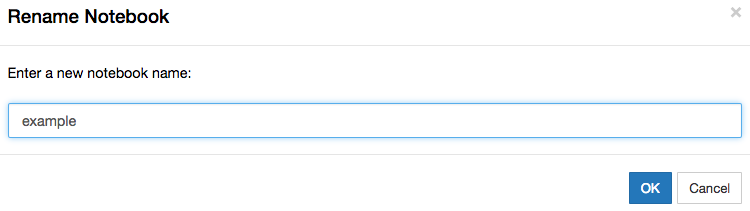
\includegraphics[width=.7\textwidth]{figures/rename_notebook.png}
\caption{Rename the notebook.}
\label{fig:rename-notebook}
\end{figure}

In the first cell, type \texttt{print("Hello World")}.
Then press Shift+Enter.
This key combination runs the cell.
A new cell will automatically appear below the cell with the print statement.
To save the notebook, hit Command+S.
Your notebook should now look like Figure \ref{fig:example-notebook}.

\begin{figure}[h]
\centering
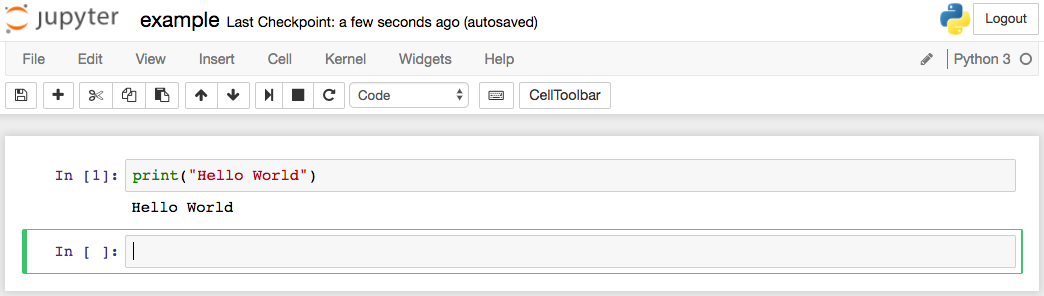
\includegraphics[width=.7\textwidth]{figures/example_notebook.png}
\caption{A Jupyter notebook.}
\label{fig:example-notebook}
\end{figure}

Now navigate to the command line where you launched Jupyter.
To stop the Jupyter server from running, hit Ctrl+c twice.
This will shut down the Jupyter notebook.
If you didn't exit the browser window yet, it will look like Figure \ref{fig:jupyter-shutdown} after you shut down the Jupyter server.
You are safe to close all browser windows related to this Jupyter notebook.

\begin{figure}[h]
\centering
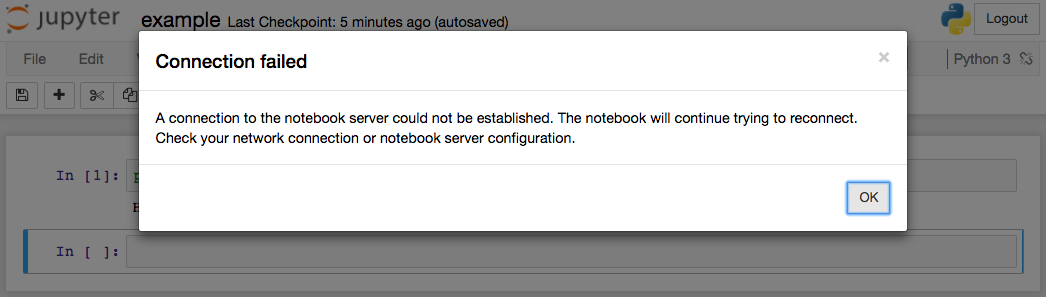
\includegraphics[width=.7\textwidth]{figures/jupyter_shutdown.png}
\caption{Shutting down a Jupyter notebook.}
\label{fig:jupyter-shutdown}
\end{figure}

\subsubsection{Committing Changes}
In the command prompt, navigate to the repository, if you aren't already there.
Type \texttt{git status} and hit enter.
You should see a message that looks similar to Figure \ref{fig:git-status}.

\begin{figure}[h]
\centering
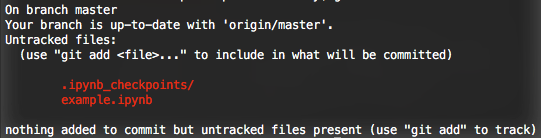
\includegraphics[width=.7\textwidth]{figures/git_status.png}
\caption{\texttt{git status}}
\label{fig:git-status}
\end{figure}

You want to add the notebook you just created to the Git index so Git knows to keep track of this file and any future changes made to it.
To do this, type \texttt{git add example.ipynb} and hit enter.
Now we are going to commit this change to the branch.
Then, type \texttt{git commit -m "example notebook"}.
A message that looks like Figure \ref{fig:git-commit} will appear.
Note that you can type any descriptive message you want in the quotes.
These messages are to help you keep track of the changes you make in each commit.
Now we want to push these changes up the master branch, so that any other machines with this repository can pull the changes you made.
Type \texttt{git push origin master} and hit enter.
Congratulations!
You have just pushed your first change to your GitHub repository.
If you navigate to the web page of your repository, you should see the example.ipynb file there, as in Figure \ref{fig:updated-repo}.

\begin{figure}[h]
\centering
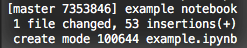
\includegraphics[width=.4\textwidth]{figures/git_commit.png}
\caption{\texttt{git commit}}
\label{fig:git-commit}
\end{figure}

\begin{figure}[h!]
\centering
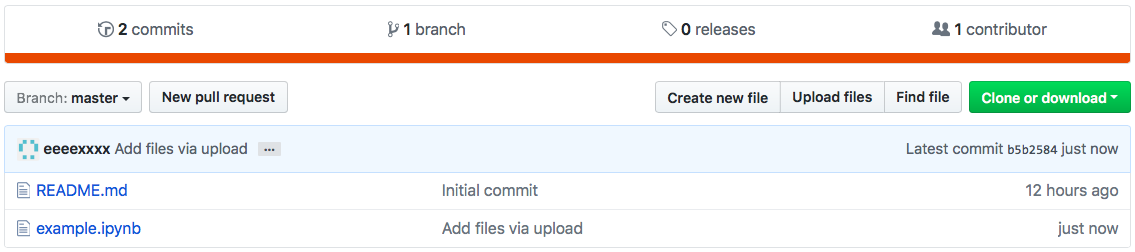
\includegraphics[width=.7\textwidth]{figures/updated_repo.png}
\caption{Updated Repository}
\label{fig:updated-repo}
\end{figure}

\subsubsection{Pulling Changes}
If you ever push a change to a repository branch on one machine, and you have the repository branch on another machine, you can still access the changes you made elsewhere.
Type \texttt{git pull origin branch\_name} to retrieve changes you have made to the branch elsewhere.

\subsection{Using the Website} \label{website}
\subsubsection{Downloading Files}
To download a file from the website of your repository, find the file you wish to download, and click on its name.
Click ``Raw" (Figure \ref{fig:download}).
This will take you to a new web page with the raw version of the file you want to download (for example, if you are trying to download a Jupyter notebook, you will see file in JSON format).
Control-click on this web page and select ``Save As...".
You can save the file anywhere you'd like on your local machine.

\begin{figure}[h!]
\centering
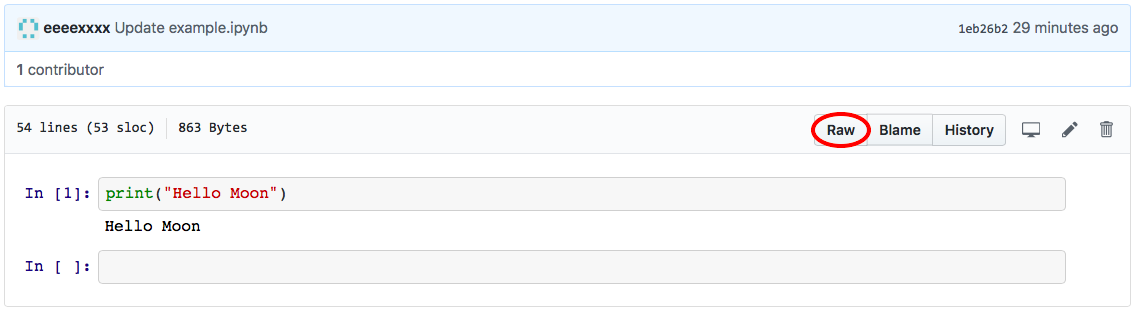
\includegraphics[width=.7\textwidth]{figures/download.png}
\caption{Download files from the website.}
\label{fig:download}
\end{figure}

\subsubsection{Uploading Files}
To upload files to your repository using the website, navigate to the main repository page and click ``Upload Files".
You can drag and drop the files you wish to upload or use a navigation tool to find them on your local machine.
Then you have two options: you can either commit those changes directly to the branch you are in, or you can commit those changes to a new branch.

\section{Forking Repositories}
Navigate to the class repository. 
The link is \url{https://github.com/tfolkman/byu_econ_applied_machine_learning}.
Click the ``Fork" button in the upper-left corner (Figure \ref{fig:fork}).
Now you have forked the repository, and it will show up in your list of repositories.

\begin{figure}[h!]
\centering

\includegraphics[width=.7\textwidth]{figures/fork.png}
\caption{Fork a Repository}
\label{fig:fork}
\end{figure}

\subsection{Updating a Fork}

Suppose a contributor of the original repository (the one from which you forked) makes a change, and you want to update your fork with that change.
To make sure you are tracking the correct remote branch, type \texttt{git remote add upstream git://github.com/pjhyett/github-services.git} in the command line.
This adds a remote (a pointer or link) to the class repository called \texttt{upstream}.
To update your fork's master branch, use the command \texttt{git pull upstream master} (make sure you are on the master branch first!).
Now your forked repository should reflect the changes made in the original repository.

\section{Deleting Repositories}
\textbf{PROCEED WITH CAUTION.}
This action cannot be undone.

To delete a repository, first navigate to the repository's main page.
Click ``Settings".
Scroll down to the bottom of the screen until you reach the ``Danger Zone".
Click ``Delete the repository".
You will have to type the name of the repository to verify that you want to completely delete it.
Then you can erase it from your GitHub.

\section{Appendix}

\subsection{List of Git Commands} \label{git-commands}

\begin{itemize}
\item \texttt{git clone repository\_link}: Clone the repository to a local machine.
\item \texttt{git status}: Display the current status of the Git index.
\item \texttt{git add filename}: Add filename to Git index to be tracked.
\item \texttt{git branch}: Check which branch you are currently on
\item \texttt{git commit -m "message"}: Commit the changes to the file or files. 
\item \texttt{git push origin branch\_name}: Submit the changes to the branch.
\item \texttt{git pull origin branch\_name}: Retrieve changes to the branch.
\item \texttt{git checkout -b branch\_name}: Create and switch to a new branch.
\item \texttt{git checkout branch\_name}: Switch to an existing branch.
\item \texttt{git branch -d branch\_name}: Delete an existing branch.
\end{itemize}

\subsection{Making New Branches}

\subsubsection{Command Line}
You might want to make different branches for different tasks.
To switch to a new, nonexistent branch, type \texttt{git checkout -b branch\_name}, where ``branch\_name" is the name you want to give the new branch.
Now you can use the previous steps to add, commit, and push changes.
The only difference is when you push, you will type \texttt{git push origin branch\_name} (instead of pushing to the master branch).
To navigate to an existing branch, type \texttt{git checkout branch\_name}, where ``branch\_name: is the name of the existing branch.
To delete an existing branch, type \texttt{git checkout -d branch\_name}.
Be careful with this last command.

\subsubsection{Using the Website}
To make a new branch on the GitHub website, navigate to the main repository page.
Click ``Branch: master".
A dropdown menu should appear (Figure \ref{create-branch}.
Start typing the name of the branch you wish to create in the text field.
An option will appear that says ``Create branch".
Click it, and you will now be on the main page for that branch.
You can use that dropdown menu to switch between branches.

\begin{figure}[h!]
\centering
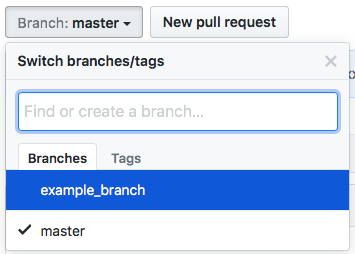
\includegraphics[width=.4\textwidth]{figures/create_branch_website.png}
\caption{Create a Branch}
\label{fig:create-branch}
\end{figure}


\subsection{Pull Requests}
If you committed on a different branch besides the master, and you want to merge these changes with the master, you can submit what is called a pull request.
Pull requests are very useful when you collaborate on a project with other people.
Pull requests allow others to see the differences between the changes you made and the branch with which you are requesting to merge.
To submit a pull request, navigate to the main screen of your repository on the GitHub website.
Click the ``Create Pull Request" button (Figure \ref{fig:pull-request}).

\begin{figure}[h!]
\centering
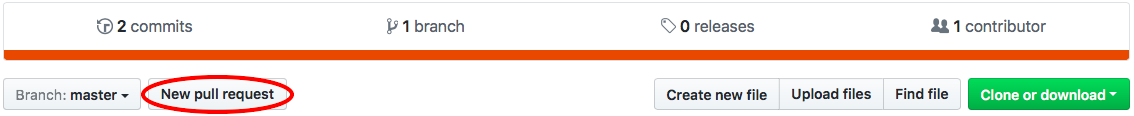
\includegraphics[width=.7\textwidth]{figures/pull_request.png}
\caption{Pull Request}
\label{fig:pull-request}
\end{figure}

This will bring you to a new screen that looks like Figure \ref{fig:pull-request2}.

\begin{figure}[h!]
\centering
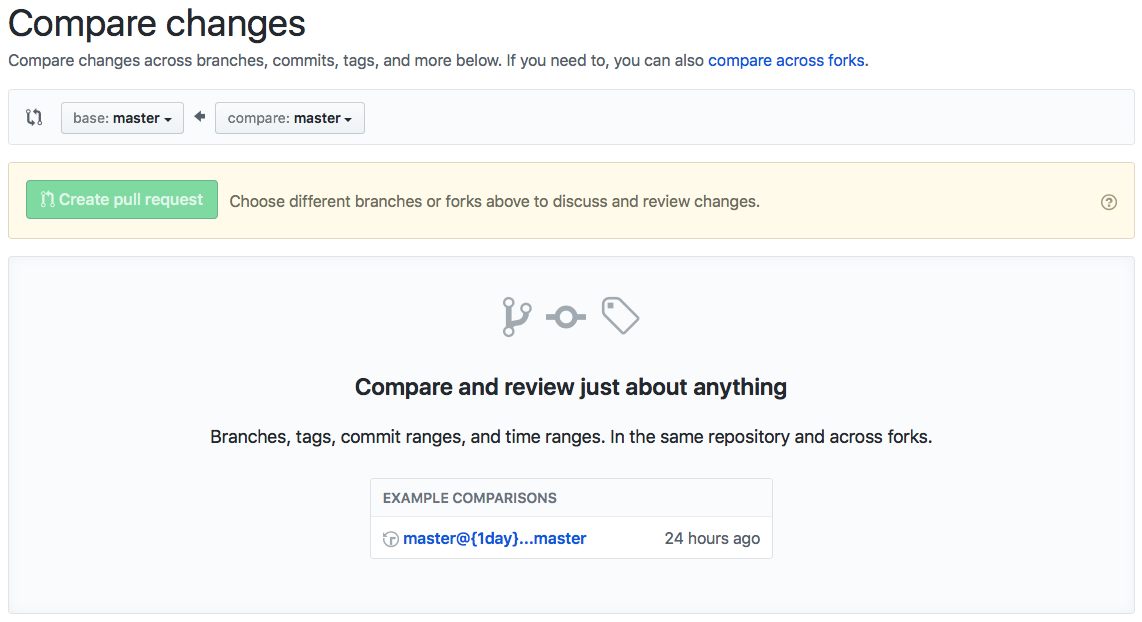
\includegraphics[width=.7\textwidth]{figures/pull_request2.png}
\caption{Pull Request}
\label{fig:pull-request2}
\end{figure}

The base branch is the branch that does not have the changes you made.
The compare branch is the branch with which you want the base branch to be merged.
For example, if you made a branch for data cleaning called data\_cleaning, and you want those changes to be reflected in the master branch, you would choose the base branch to be master, and the compare branch to be data\_cleaning.
Once you have chosen the appropriate branches, click ``Create Pull Request".
Then you will see a page that looks like Figure \ref{fig:open-pull-request}.

\begin{figure}[h!]
\centering
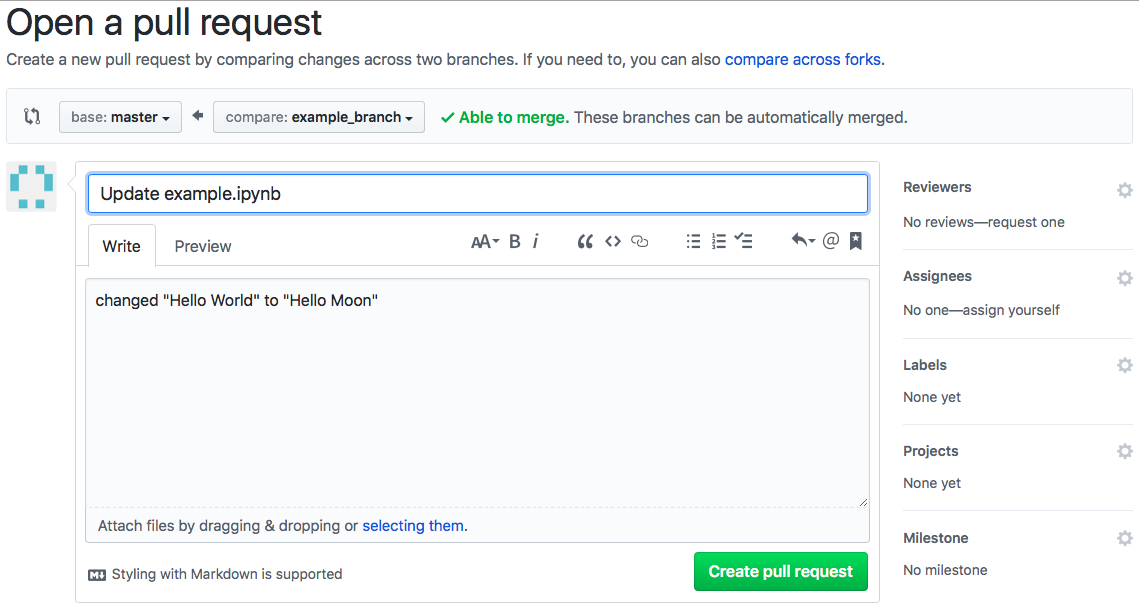
\includegraphics[width=.7\textwidth]{figures/open_pull_request.png}
\caption{Pull Request}
\label{fig:open-pull-request}
\end{figure}

In the ``Write" section, it is helpful if you describe what you changed.
In a collaboration project with dozens of files and thousands of lines of code, it is helpful to other reviewers to see an outline of what you changed at a glance.
If you scroll down, you will see sections that describe what has been changed and what is different between the two branches.
You can request reviewers, and you and other collaborators can make comments about changes.
When you are ready to make the pull request official, click ``Create Pull Request".
After clicking this, you will see a web page that looks like Figure \ref{fig:open-pull-request2}.

\begin{figure}[h!]
\centering
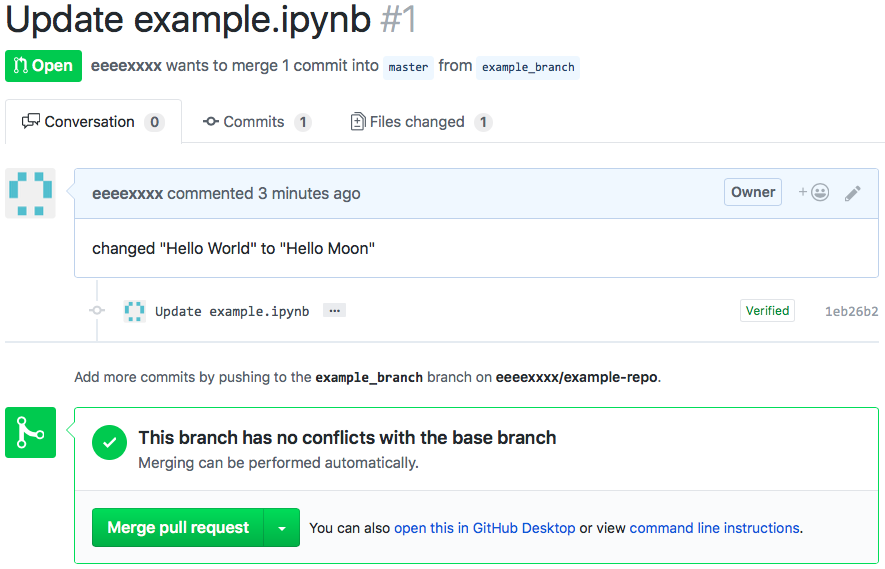
\includegraphics[width=.7\textwidth]{figures/open_pull_request2.png}
\caption{Pull Request}
\label{fig:open-pull-request2}
\end{figure}

When you and/or your collaborators have reviewed your changes and are ready to merge them to the base branch (and the compare branch has no conflicts with the base branch), click ``Merge Pull Request".
After the branches are merged, you are safe to delete the compare branch.

\end{document}
